% 両面印刷する場合は `openany' を削除する
\documentclass[openany,11pt,papersize]{jsbook}

%パッケージの読み込みなど
% 報告書提出用スタイルファイル
\usepackage[final]{funpro}%最終報告書
%\usepackage[middle]{funpro}%中間報告書

% 画像ファイル (EPS, EPDF, PNG) を読み込むために
\usepackage[dvipdfmx]{graphicx,color}

%数式の表示に利用するため
\usepackage{amsmath,amssymb}

%アルゴリズムの表示に利用するパッケージ
\usepackage{algorithm}
\usepackage{algorithmic}

%枠をつけるためのパッケージ
\usepackage{ascmac}

%図の位置調整パッケージ
\usepackage{here}

%付録を作成するためのパッケージ
\usepackage{appendix}

%ドキュメント管理用パッケージ
\usepackage{docmute}


% ここから -->
\usepackage{calc,ifthen}
\newcounter{hoge}
\newcommand{\fake}[1]{\whiledo{\thehoge<70}{#1\stepcounter{hoge}}%
  \setcounter{hoge}{0}}
% <-- ここまで 削除してもよい


% 年度の指定
\thisYear{2016}

% プロジェクト名
\jProjectName{FUN-ECM プロジェクト}

% [簡易版のプロジェクト名]{正式なプロジェクト名}
% 欧文のプロジェクト名が極端に長い(2行を超える)場合は,短い記述を
% 任意引数として渡す.
%\eProjectName[Making Delicious curry]{How to make delicious curry of Hakodate}
\eProjectName{FUN-ECM Project}


% <プロジェクト番号>-<グループ名>
\ProjectNumber{15-A}

% グループ名
\jGroupName{Aグループ}
\eGroupName{A Group}

% プロジェクトリーダ
\ProjectLeader{1014129}{池野竜將}{Ryusuke Ikeno}

% グループリーダ
\GroupLeader  {1014129}{池野竜將}{Ryusuke Ikeno}

% メンバー数
\SumOfMembers{8}
% グループメンバ
\GroupMember  {1}{1014068}{駒ヶ嶺壮}{Sou Komagamine}
\GroupMember  {2}{1014109}{伊藤有輝}{Yuki Ito}
\GroupMember  {3}{1014129}{池野竜將}{Ryusuke Ikeno}
\GroupMember  {4}{1014137}{千葉大樹}{Daiju Chiba}
\GroupMember  {5}{1014164}{橋本和典}{Kazunori Hashimoto}
\GroupMember  {6}{1014168}{山下哲平}{Teppei Yamashita}
\GroupMember  {7}{1014209}{源啓多}{Keita Minamoto}
\GroupMember  {8}{1013150}{亀谷浩也}{Hiroya Kametani}

% 指導教員
\jadvisor{白勢政明,由良文孝}
% 複数人数いる場合はカンマ(,)で区切る.カンマの前後に空白は入れない.
\eadvisor{Masaaki Shirase, Fumitaka Yura}

% 論文提出日
\jdate{2016年7月27日}
\edate{July~27, 2016}


\begin{document}

\chapter{後期活動内容}
後期の活動は,前期の活動に加えて広報活動を行った.また,理論班には作成したプログラムの検証を行った.
\bunseki{亀谷浩也}

\section{理論班}
\label{sec:theoryresult}
理論班は,新たに取り入れた理論とプログラム班によって実装されたプログラムがどれほど高速化されたのかを検証した.

\subsection{活動目的}
ECMプログラムの効率化は本プロジェクトの目的であるECMNETへのランクインに必要不可欠な要素である.効率化のために取り入れたプログラムが処理時間にどのような影響がでるのかを調べることは今後プログラムを改善していくうえで重要な項目である.
今回は昨年度に使用されたECMプログラムと今年度のプログラムの比較評価を行った.昨年度と今年度のプログラムの主な違いは,スカラー倍算の高速化(kP)アルゴリズムの実装,Atkin-Morain ECPPの実装,そしてStage2の実装である.この実装によりECMプログラムの素因数発見の効率を上げ,処理速度の向上に貢献したと予想をふまえて,今年度のプログラムが昨年度よりどのように改善されたのかを検証する.またこの変更がプログラムにどのような効果をもたらすかを知ることで,今後のプログラムの改善に役立つことができる.

\subsection{活動内容}
 検証班は今年度にプログラミング班が作ったプログラムと昨年度のプログラムを実行しどれだけ改善したかを検証することにした.今回は素因数分解アルゴリズムの処理速度を評価したいと考えた.今年度のECMプログラムでは素因数の発見確率を上げたことから素数ではなく合成数を入力することにした.検証結果を統計的に信憑性を持たせるためにいくつかの統計方法を調べた.しかし,どの検証方法も今回の検証に適切ではないと判断した.そこで今年度は20桁から50桁の合成数を5桁刻みで各5回ずつ入力し,各桁の処理時間のトータルタイムの平均時間を比較した.しかし一回プログラムを検証するのに3時間かかるものもある上に学内でしか検証ができないことから統計的には検証回数が少なく信憑性の低い結果になった.検証環境については学内のサーバーを利用し,以下の通りである.
 
\begin{itembox}[l]{検証環境}
コンパイラ: icc 14.0.1

OpenMP   : 3.1

GMP       : 6.0.0

CPU    : Intel Xeon Phi 5110P(60コア)

RAM   : 64GB(DDR3L-1600 8GB DIMM×8)

  \end{itembox}

\subsection{検証結果}
検証結果のまとめは以下の表のようになった.

\begin{table}[htb]
  \begin{tabular}{|l|r|r||l|} \hline
    桁数 & 今年度(秒) & 昨年度(秒) & 平均改善率 \\ \hline \hline
    20 & 3.400~3.696             & 1.689~2.257             & -82\% \\ \hline
    25 & 10.906~11.323          & 8.528~9.513             & -25\% \\ \hline
    30 & 47.165~51.537          & 44.223~47.599          & -4\% \\ \hline
    35 & 177.932~190.253       & 191.348~200.441       & +6\% \\ \hline
    40 & 686.793~693.397       & 711.594~713.633       & +4\% \\ \hline
    45 & 2682.470~2745.112    & 2653.112~2667.896    & +0\% \\ \hline
    50 & 10173.577~10622.231 & 11763.204~11849.030 & +12\% \\ \hline
  \end{tabular}
\end{table}
20桁から30桁では今年度のプログラムの平均改善率は昨年度より下回る結果になったが35桁以降は徐々に上がっていき最大15%も改善し処理速度が速くなった.
上述の通り,本プロジェクトの目的である巨大な桁数の合成数を素因数分解するのに昨年度のプログラムより改善した.したがって素因数発見確率を上げたことによって処理速度を向上させたことを証明した.
\bunseki{亀谷浩也}

\section{プログラミング班}
プログラミング班は前期の活動に引き続き,ECMプログラムの改善を行った.
\bunseki{亀谷浩也}

\subsection{Atkin-Morain ECPPの実装}
後期にまず行ったのはAtkin-Morain ECPPの実装だ.このアルゴリズムは前期中に理論班によって提示されたものだ.詳細なアルゴリズムは\ref{sec:ECPP}に記述した.
\bunseki{亀谷浩也}

\subsection{スカラー倍算の高速化}
Atkin-Morain ECPPを実装後,私たちは楕円曲線上の点のスカラー倍算の高速化に取り組んだ.スカラー倍算はECMのアルゴリズムの中で最も計算量の多い箇所の為,高速化が期待できると考えたからだ.そのために,移動窓法(sliding/moving window method)を実装した.移動窓法はバイナリ法(binary method)やm進展開法(window method),符号付きm進展開窓法などと比較される楕円曲線演算の高速化手法だ.移動窓法の理解に際し,バイナリ法及びm進展開法について学んだので,まずはこれらについて記述する.
\bunseki{源啓多}

\subsubsection{バイナリ法}
バイナリ法は楕円曲線上の点$Pをk倍した点kPを求める際に,k$を2進展開することで,高速なスカラー倍算を実現する手法である.昨年度から引き継いだプログラムでは,このアルゴリズムが採用されていた.バイナリ法の詳細なアルゴリズムを以下に示す.

\begin{algorithm}[H]                   
\caption{binary method}
\label{alg:algB}                          
\begin{algorithmic}                  
\REQUIRE $P, n$bit integer $k = {\displaystyle \Sigma_{i=0 \rightarrow n-1}}k_j 2^j$,$k_j \in \{0,1\}$
\ENSURE $Q = kP$
\STATE $P_1 \leftarrow P$
\FOR {$i = 2$ to $m-1$}
\STATE $P_i \leftarrow P_{i-1} + P$
\ENDFOR
\STATE $Q \leftarrow 0$
\FOR {$j=d-1$ to $0$ by $-1$}
\STATE $Q \leftarrow mQ$
\STATE $Q \leftarrow Q+P_{k_j}$
\ENDFOR
\end{algorithmic}
\end{algorithm}

バイナリ法を用いなかった場合,$kPを計算する手順はP+P+P+…+Pであり,これには加算がk-1$回必要である.対して,バイナリ法を用いた場合は加算と2倍算がそれぞれ回で済む.したがって,バイナリ法を採用することで大きいkに対して高速にスカラー倍算を行うことができる.

\bunseki{源啓多}

\subsubsection{m進展開法}
 $m$進展開法では,バイナリ法を応用して,2進展開ではなく$m進展開を行っている.m進展開の容易さから,mは2^r(r\in Z, r>Z)のような値であることが多い.事前計算として2P, 3P, ・・・, (m-1)Pを計算する必要があるが,
であるとき,rビット単位で計算を行うことができるので,高速化につながる.以下は,m進展開法のアルゴリズムである.$

\begin{algorithm}[H]                   
\caption{window method}
\label{alg:algW}                          
\begin{algorithmic}                  
\REQUIRE $P, k = \Sigma_{i=0\rightarrow d-1}k_j m^j, k_j\{0,1, ... , m-1\}$
\ENSURE $Q = kP$
\STATE $P_1 \leftarrow P$
\FOR {$i =2$ to $m-1$}
\STATE $P_i \leftarrow P_{i-1} + P$
\ENDFOR
\STATE $Q \leftarrow 0$
\FOR {$j=d-1$ to $0$ by $-1$}
\STATE $Q \leftarrow mQ$
\STATE $Q \leftarrow Q+P_{k_j}$
\ENDFOR
\end{algorithmic}
\end{algorithm}

\bunseki{源啓多}

\subsubsection{移動窓法}
 $m進展開法をさらに発展させたのが移動窓法である.移動窓法では,計算を行う単位をr$ビットに固定しておらず,末尾のビットが1かつ$r$ビット以下で最長になるような単位で計算を行う.末尾のビットが1であるようにすることで,事前計算の量が$m$進展開法に比べて半分で済むことが移動窓法の特徴である.移動窓法のアルゴリズムを以下に示す.
 
\begin{algorithm}[H]                   
\caption{moving/sliding window method}
\label{alg:algW}                          
\begin{algorithmic}                  
\REQUIRE $P, k=\Sigma_{i=0 \rightarrow n-1}k_j 2^J,k_j \in \{0,1\}$
\ENSURE $Q=kP$
\STATE $P_1 \leftarrow P$
\STATE $P_2 \leftarrow 2P$
\FOR {$i=1$ to $2^{r-1} -1$}
\STATE $P_{2i+1} \leftarrow P_{2i-1}+P_2$
\ENDFOR
\STATE $j \leftarrow n-1$
\STATE $Q \leftarrow 0$
\WHILE {$j \geq 0$}
\IF {$k_j = 0$}
\STATE $Q \leftarrow 2Q$
\STATE $j \leftarrow j-1$
\ELSE
\STATE $t= \min \{ j-t+1 \leq r AND k_t = 1 \}$
\STATE $h_j \leftarrow ( k_j, k_{j-1},  \cdots , k_t)_2$
\STATE $Q \leftarrow [2^{j-t+1}]Q + P_{h_j}$
\STATE $j \leftarrow t-1$
\ENDIF
\ENDWHILE
\end{algorithmic}
\end{algorithm}

他に採用するアルゴリズムとして,移動窓法の実装後にMontgomery ladderが挙がったが,実装・比較する期間を設けられなかったので来年度への課題とする.

\subsection{Stage2}
前述したようなアルゴリズムを調査した結果,現状のアルゴリズムを改善するより新たなアルゴリズムを導入することが良いと考え,後期ではStage2というアルゴリズムを実装した.まず,Stage2の前提として,Stage1を説明する.Stage1は,Pのk倍,すなわちkPを計算する過程である.具体的には,以下のような手順でkを決定し,計算を行っている.

\begin{itembox}[l]{Stage1}
\begin{center}
\[
k = \prod_{2 \leq p \leq B_1, p \in \mathbb{P}} p^{\lfloor \log{p} B_1 \rfloor}
\]
\end{center}
\end{itembox}

前述の式で求めた$kを利用してkP$を計算し,$kPのx$座標と合成数の最大公約数をとる.その結果最大公約数が1でなければ素因数分解が成功したことになる.しかし,Stage1だけでは,$B_1$より大きい素数を1つだけ$kP$にかけていれば,素因数が求まった,ということが起こりうる.Stage2は,これの頻度を減らすためのアルゴリズムである.Stage2のための新たなパラメータ$B_2(> B_1)$を設定し,$B_1より大きく,B_2$以下の素数$p’$それぞれをStage1の計算結果kPにかけ,それぞれの$p’(kP)$のx座標と合成数Nの最大公約数を計算する.もし計算結果が1でなければ,素因数が求められたことになる.
\bunseki{源啓多}

\subsubsection*{基本的なStage2の実装}

\begin{algorithm}[H]                   
\caption{Basic ECM Algorithm}
\label{alg:B}                          
\begin{algorithmic}                  
\REQUIRE $N$ is composite number, $E$ is elliptic curve, $P = (x_0, y_0, Z_0) \in E(Z_n)$ is initial point, $B_1$ is smoothness bound for Phase 1, $B_2$ is smoothness bound for Phase 2, $B_2 \ge B_1.$
\ENSURE $q$ is factor of $N$, $1 \le q \leq N$, or FAIL.
\STATE \bfseries{Phase 1.}
\STATE $k \gets \prod_{p \leq B_1} p^{\log{p} B_1}$
\STATE $Q_0 \gets kP_0$
\STATE $q \gets \gcd(z_{Q_0},N)$
\IF {$q \ge 1$}
\STATE return $q$
\ELSE
\STATE go to Phase 2
\ENDIF
\STATE \bfseries{Phase 2.}
\STATE $d \gets 1$
\FOR {each prime $p = B_1$ to $B_2$} 
\STATE $(x_{pQ_0},y_{pQ_0},z_{pQ_0}) \gets pQ_0$
\STATE $d \gets d*Z_{pQ_0} (mod N)$
\ENDFOR
\STATE $q \gets \gcd(d,N)$
\IF {$q \ge 1$}
\STATE return $q$
\ELSE
\STATE return FAIL
\ENDIF
\end{algorithmic}
\end{algorithm}

\bunseki{源啓多}

\subsection{開発環境と実行環境}
プログラムを実行する環境について記述する.前期までは,Xeon Phi 5110Pを用いてプログラムを実行していたが,Xeon E5-2640で実行した方がプログラムの実行速度が速かったため,Xeon E5-2640を主に使用することにし,Xeon Phi 5110Pは検証用に使用することにした.メインメモリについては,64GB(DDR3L-1600 8GB DIMM×8)を搭載している.コンパイラはicc 14.0.1,OpenMPのバージョンは3.1,GMPは6.0.0を使用している.コンパイル時には,最適化オプション(-O2)を指定している.

\subsection{GMPについて}
ECMをC言語で実装するにあたり,符号なし64bitの数値型であるunsigned long longを用いてもオーバーフローすることは避けられない.そのため,多倍長計算を高速に行うライブラリであるGMPを使用した.GMPで使用した関数について説明する.

\begin{description}
 \item[void mpz\_init(mpz\_t x)]\mbox{}\\ 
mpz\_init()はmpz\_t型の変数xを初期化するための関数である.

\item[void mpz\_inits(mpz\_t x, …)]\mbox{}\\ 
mpz\_inits()は複数のmpz\_t型の変数を初期化するための関数である.引数として与えられた変数のリストは,NULLで終端しなければならない.

\item[void mpz\_clear(mpz\_t x)]\mbox{}\\ 
mpz\_clear()はmpz\_t型の変数xが確保していたメモリを開放するための関数である.

\item[void mpz\_clears(mpz\_t x, …)]\mbox{}\\ 
mpz\_clears()は複数のmpz\_t型の変数が確保していたメモリを開放するための関数である.引数として与えられた変数のリストは,NULLで終端しなければならない.

\item[void mpz\_set(mpz\_t rop, const mpz\_t op)]\mbox{}\\ 
mpz\_set()はmpz\_t型の変数の代入を行う関数である.mpz\_set\_ui(),mpz\_set\_si(),などのバージョンがあり,それぞれ第2引数がunsigned long int,signed long intになっている.mpz\_set\_str()という関数もあり,第2引数がconst char*になっており,第3引数には基数を指定する.そして,第2引数に指定した文字列を第3引数に指定した基数に基づき,整数だと解釈して第1引数に指定したmpz\_t型の変数に代入する.

\item[void mpz\_add(mpz\_t rop, const mpz\_t op1, const mpz\_t op2)]\mbox{}\\ 
op1+op2をropに代入する.第3引数の型がunsigned long intであるmpz\_add\_uiも存在する.

\item[void mpz\_sub(mpz\_t rop, const mpz\_t op1, const mpz\_t op2)]\mbox{}\\ 
op1-op2をropに代入する.第3引数の型がsigned long intであるmpz\_sub\_si(),unsigned long intであるmpz\_sub\_ui()も存在する.

\item[void mpz\_mul(mpz\_t rop, const mpz\_t op1, const mpz\_t op2)]\mbox{}\\ 
op1*op2をropに代入する.第3引数の型がsigned long intであるmpz\_mul\_si(),unsigned long intであるmpz\_mul\_ui()も存在する.
	
\item[void mpz\_pow\_ui(mpz\_t rop, const mpz\_t base, unsigned long int exp)]\mbox{}\\ 
baseをexp乗し,ropに代入する.

\item[void mpz\_mod(mpz\_t r, const mpz\_t n, const mpz\_t d)]\mbox{}\\ 
n mod dをrに代入する.
\end{description}

\section{広報班}
広報班では,プロジェクト活動や楕円曲線法の解説を外部に発信することにした.発信をする方法として,FUN-ECMのWEBページを制作することにした.WEBサイトを制作するにあたって後期の活動から広報班を新たに結成し,活動を行った.発信する対象は主に情報系の大学生とし,学部一年生の知識でも理解できるように楕円曲線法とその周辺の理論的な基礎知識を表記した.また,来年度以降の活動や,専門知識をもった人にむけて今年得た知識やプログラムで変更した点など,今年度の専門的な活動内容も表記した.
\bunseki{亀谷浩也}

\subsection{動機}
FUN-ECMは今年で3年目であるが,毎年ECMのプログラムの改良を重ねる活動であるため毎年外部への露出が少なく,継続性の強いプロジェクトであることから私たちは今年度ならではの対外的な新規活動をしたいと考えた.新規的な活動をするにあたり,未来大生でもECMについて知らない方が多いことからより多くの人にECMを伝えられるように広報的活動を行うことにした.また,中間発表での意見でプレゼンでは理解しにくかったとの意見を頂いたことからよりわかりやすく伝えられ,手軽にみることができる媒体としてwebページを採用した.

\bunseki{駒ヶ嶺壮}

\subsection{Webページの構成と内容}
\subsubsection{Top}
本サイトのトップページ.SNSの共有ボタン,活動写真のスライダーやFUN-ECMとは何かに関する簡単な説明がある.また,ここでは来年度の活動のためのアンケートページも設置した.一番下にあるボタンから各ページに飛ぶことができる.

\bunseki{亀谷浩也}

\subsubsection{About}
広報班が活動目的としていた内容のコンテンツである.ECMの基礎理論の説明ページ,FUN-ECMの活動目的,今年度のECMプログラムの解説ページの3つに分かれている.章ごとに分けて詳細的な説明を行い,段階的に読み進めることができるようにした.また,重要な箇所での色の変更やgif画像を挿入するなどしてより理解しやすいように工夫した.ECMプログラムの解説ページでは今年度のプログラムのソースコードの一部を掲載し,すべてのソースコードについてはURLからgithubのページに飛ぶことができるようにした.

\bunseki{亀谷浩也}

\subsubsection{History}
2016年度の活動月表を掲載した.前期活動と後期活動の2つに分けて,後期活動の中には2016年度の全体成果についても記載した.どの班がどのような活動をしたかについて簡単にわかるようにした.

\bunseki{亀谷浩也}

\subsubsection{Link}
リンク集.本プロジェクトで使用したECM-NETや本学のホームページ等を掲載した.

\bunseki{亀谷浩也}

\subsection{Webページ内のファイルの説明}

\subsubsection{bootstrap.css}
Webサイトやwebアプリケーションを作成するためのwebアプリケーションフレームワークである.Class属性を指定するだけで簡単に豊富なスタイルを指定することができるファイル.

\subsubsection{bootstrap.min.css}
bootstrap.cssの圧縮版であるファイル.読み込みを早くしたい時などはbootstrap.cssではなくこちらを使用する.

\subsubsection{jquery.bxslider.css}
スライドショー形式で表示された画像のスタイルを指定しているファイル.

\subsubsection{jsxgraph.css}
javascriptを用いた楕円曲線のグラフのスタイルをしているファイル.

\subsubsection{original.css}
上記以外のスタイルを指定している.レイアウトのために私たちが設定した

\subsubsection{bootstrap.js}
bootstrapのjavascriptの部分を動かすためのファイル.後述するjQueryのファイルを先に読み込まなければ機能しない.

\subsubsection{bootstrap.min.js}
 bootstrap.jsの圧縮版であるファイル.読み込みを早くしたい時などはbootstrap.jsではなくこちらを使用する.

\subsubsection{jquery.bxslider.min.js}
画像をスライドショー形式で表示するための関数を組み込んでいるファイルである.

\subsubsection{jquery.js}
jQueryをWEBページ内に組み込むためのファイル.jQueryとはjava scriptをより扱いやすくしたファイルであり,本来であれば複雑なプログラムの記述もjQueryを用いることで簡易的に記述することができる.

\subsubsection{jquery.min.js}
jquery.jsの圧縮版であるファイル.読み込みを早くしたい時などはjquery.jsではなくこちらを使用する.

\subsubsection{jsxgraphcore.js,GeonextReader.js}
webページ内のグラフを動かすためのjavascriptが記述されたファイル.

\subsubsection{ecm.html}
FUN-ECMウェブサイトの"ECMとは"について書かれているhtmlファイルである.「ECMとは何か」について,基礎知識として$modN$の説明や点同士に置ける加算と2倍算についての説明が記述されている.

\begin{figure}[H]
  \begin{center} %センタリングする
    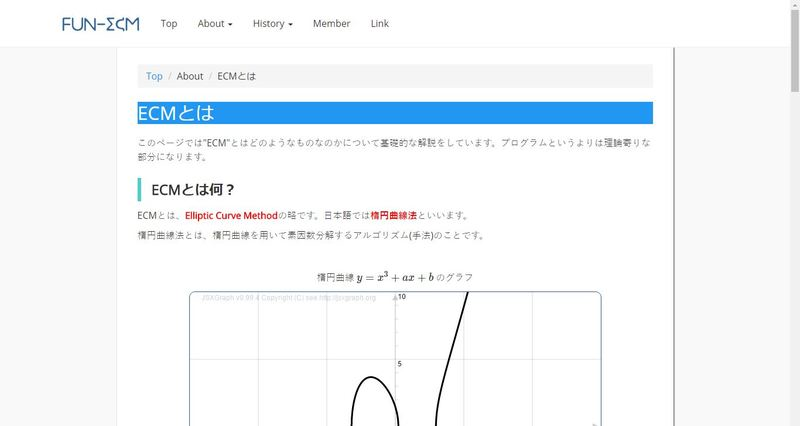
\includegraphics[clip, width=10.0cm]{./figure/ecm.png}
    \caption{ecm.html} %タイトルをつける
    \label{ecm} %ラベルをつけ図の参照を可能にする
  \end{center}
\end{figure}

\subsubsection{ecm1.html}
FUN-ECMウェブサイトの"活動目的"について書かれているhtmlファイルである.FUN-ECMがなぜ素因数分解をするのか,またECM-NETとは何かについて記述されている.

\begin{figure}[H]
  \begin{center} %センタリングする
    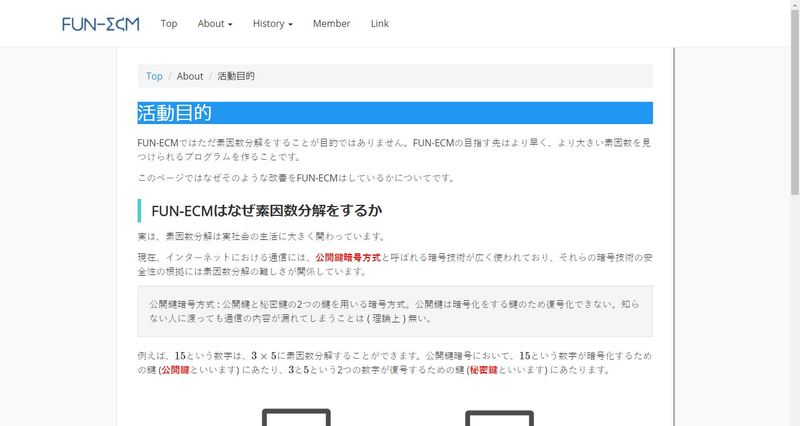
\includegraphics[clip, width=10.0cm]{./figure/ecm1.png}
    \caption{ecm1.html} %タイトルをつける
    \label{ecm1} %ラベルをつけ図の参照を可能にする
  \end{center}
\end{figure}

\subsubsection{index.html}
FUN-ECMウェブサイトの"トップページ"について書かれているhtmlファイルである.FUN-ECMの活動風景の写真や名前の由来,各ページへのリンクが記述されている.

\begin{figure}[H]
  \begin{center} %センタリングする
    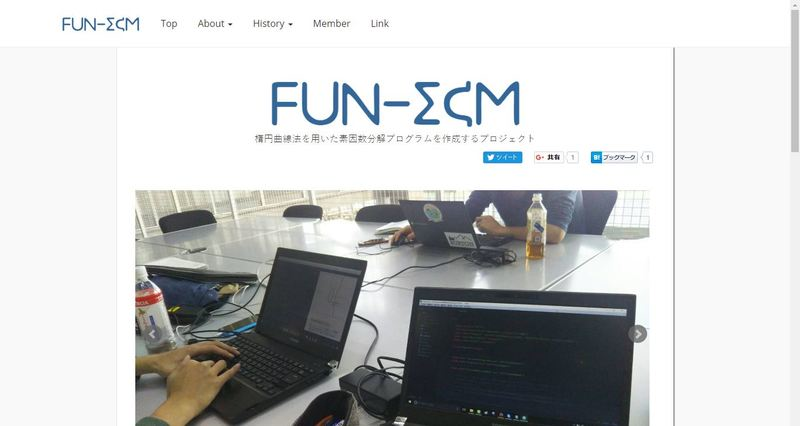
\includegraphics[clip, width=10.0cm]{./figure/index.png}
    \caption{index.html} %タイトルをつける
    \label{index} %ラベルをつけ図の参照を可能にする
  \end{center}
\end{figure}

\subsubsection{link.html}
FUN-ECMウェブサイトの"リンク"について書かれているhtmlファイルである.ECM-NETやSTUDIO KAMADAなど,ECMに関係するサイトやECMについての説明がされているサイト,またFUN-ECMの教授へのリンクも記述されている.

\begin{figure}[H]
  \begin{center} %センタリングする
    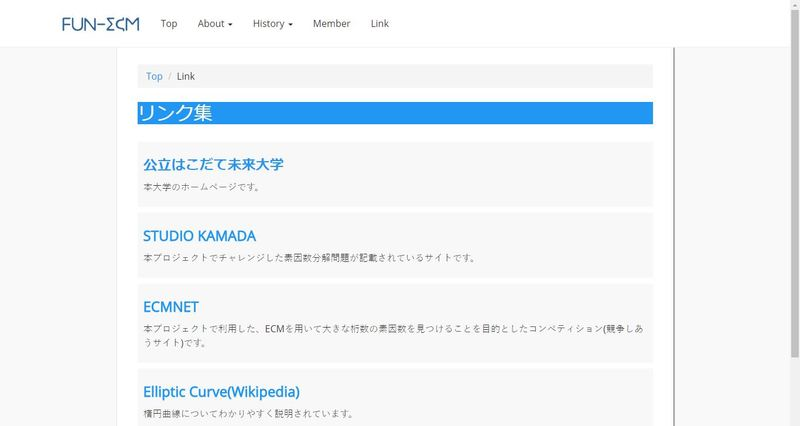
\includegraphics[clip, width=10.0cm]{./figure/link.png}
    \caption{link.html} %タイトルをつける
    \label{link} %ラベルをつけ図の参照を可能にする
  \end{center}
\end{figure}

\subsubsection{log.html}
FUN-ECMウェブサイトの"前期活動"について書かれているhtmlファイルである.4月から8月までのFUN-ECMの活動記録が記述されている.

\begin{figure}[H]
  \begin{center} %センタリングする
    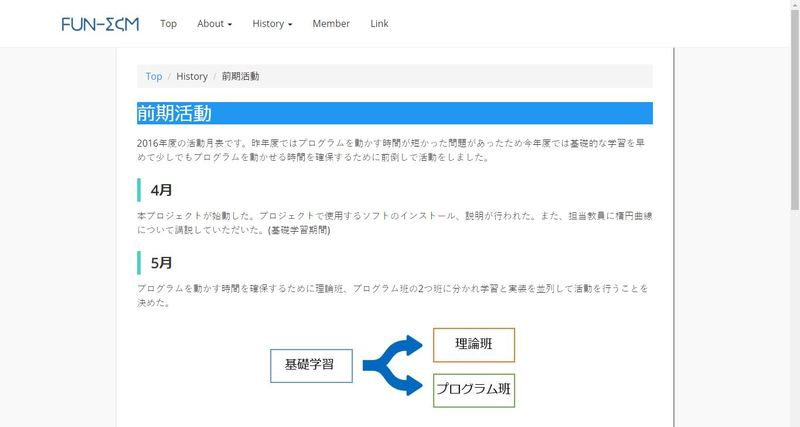
\includegraphics[clip, width=10.0cm]{./figure/log.png}
    \caption{log.html} %タイトルをつける
    \label{log} %ラベルをつけ図の参照を可能にする
  \end{center}
\end{figure}

\subsubsection{log2.html}
FUN-ECMウェブサイトの"後期活動"について書かれているhtmlファイルである.9月から1月までのFUN-ECMの活動記録が記述されている.

\begin{figure}[H]
  \begin{center} %センタリングする
    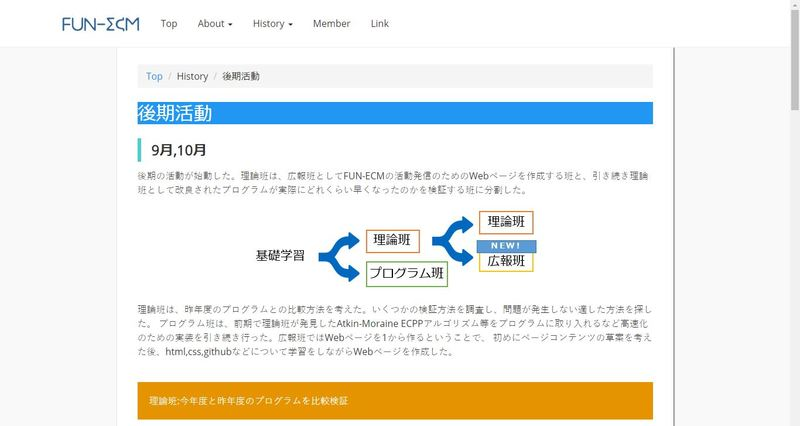
\includegraphics[clip, width=10.0cm]{./figure/log2.png}
    \caption{log2.html} %タイトルをつける
    \label{log2} %ラベルをつけ図の参照を可能にする
  \end{center}
\end{figure}

\subsubsection{member.html}
FUN-ECMウェブサイトの"メンバー紹介"について書かれているhtmlファイルである.メンバー全員の名前と班,一言が記述されている

\begin{figure}[H]
  \begin{center} %センタリングする
    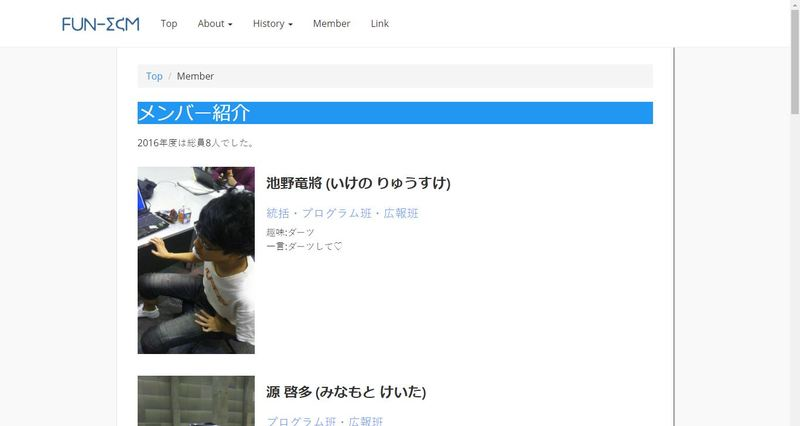
\includegraphics[clip, width=10.0cm]{./figure/member.png}
    \caption{member.html} %タイトルをつける
    \label{member} %ラベルをつけ図の参照を可能にする
  \end{center}
\end{figure}

\subsubsection{program.html}
 FUN-ECMウェブサイトの"プログラムについて"について書かれているhtmlファイルである.FUNECMプログラムの使い方やECMの基本的な実装,さらにその他のECMに関する専門的な知識やそのプログラムが記述されている.

\begin{figure}[H]
  \begin{center} %センタリングする
    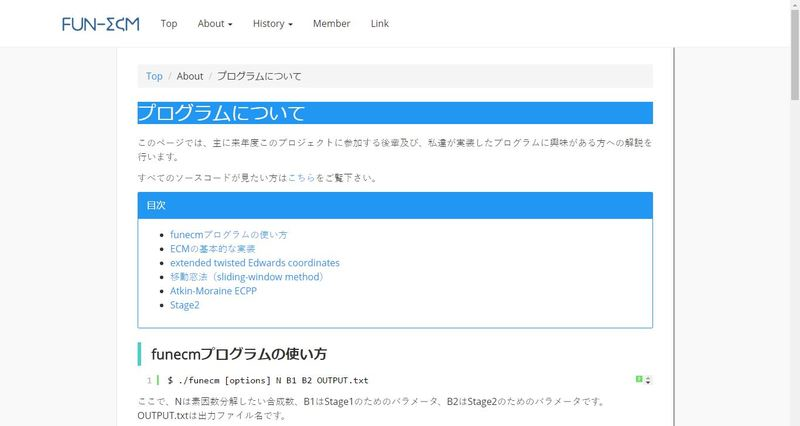
\includegraphics[clip, width=10.0cm]{./figure/program.png}
    \caption{program.html} %タイトルをつける
    \label{program} %ラベルをつけ図の参照を可能にする
  \end{center}
\end{figure}

\bunseki{亀谷浩也}

\subsection{展望}
私たちは当初,情報大学生の学部1年生でも私たちの活動を理解することのできるような解説ページを設けるという一つの目標を立て,実際にECMについての大まかな流れを難しいと思われる部分を噛み砕きつつ解説したページを作成した.そして最終発表会において私たちの発表を見てもらった方にウェブページにあるアンケートで感想を答えてもらった.しかし,アンケートに答えてもらった方の母数が少なかったため,来年度はアンケートに答えてもらう人数を今年度より増やすことによって正確な理解度の調査を行い,その結果を使いウェブページの改善を行いたい.

\section{成果発表}
成果発表会では,前期に行った中間発表のレビューを元に改善をした.レビューでは,内容が理解できた人とできていない人が分かれていたため,さらに前提知識のない聴衆にも伝わるような内容を目指した.

\subsection{準備}
\begin{description}
\item[ポスター]\mbox{}\\
後期の活動では,3つの活動を並行して行っていたため,ポスターを前期に比べて1枚増やし3枚で構成を考えた.次にメインポスターとサブポスターを分け,メインは全体の活動を大まかに伝える,サブポスターはそれぞれの活動を具体的に伝えるという目標を設定し,各自作成をした.ポスターの作成には前年度に引き続き「Microsoft PowerPoint」というソフトウェアを利用した.ポスターが完成次第,グループごとにレビューを行い,誤字脱字を修正した.
\bunseki{亀谷浩也}

\item[プレゼンテーション資料]\mbox{}\\
前期の中間発表のレビューでは,伝わった人と伝わらなかった人が分かれていたため,前提知識が殆どない聴衆でもわかりやすくなるように,専門的な用語を最小限にするように注意し,最も大事でなところを枠で囲み,その中身を見るだけで大まかな内容を理解できるようにした.また,楕円曲線法についての説明では,例示を多く含めることで数学に抵抗のある人でも触れやすいようにした.加えて,長い数式に関しては説明を省きスライドに表示するだけにとどめ,数学が苦手だという方の抵抗を減らすようにした.作成には前年度に引き続き「Microsoft PowerPoint」というソフトウェアを利用した.
\bunseki{亀谷浩也}

\end{description}

\subsection{発表}
発表は,前後半で4人ずつに分かれて行った.前半は3人がそれぞれの担当について発表を行い,1人がポスターの前で質問を受けたり,評価シートを配るという配役で行った.後半は4人がそれぞれの担当について発表を行い,発表を行っていない1人が他の作業を行った.前期の発表中にプロジェクターの電源が落ちてしまうアクシデントがあった為,そのようなアクシデントに対応するために,PCでプレゼンテーションを行いながら復旧作業を行うことを決めた.発表後に評価アンケートの集計を行った結果,発表技術は10点中平均7.1点,発表内容は10点中7.9点だった.共に前期の評価よりも点数が上昇しており,発表の工夫の効果が表れていることが確認できた.しかし,いくつかのコメントに内容を省きすぎている,数式の説明をしないのはよくない,などの意見もあった.

\bunseki{亀谷浩也}
\end{document}
